\subsection*{Data and Variable Descriptions}
In our neuroimaging experiments, a large number of our features describe specific and localized regions of the brain across multiple imaging modalities. Below we list and describe each of regions for each modality, and give a brief background on each of methods used to acquire the data. We also include the list of cognitive scores used in our analysis.

\subsubsection*{PET Imaging}
Positron emission tomography has become an increasingly popular method of imaging the brain, specifically in the areas where cognitive decline can be strongly correlated with the specific matter being imaged. Pittsburgh compound B (PiB) was used as the tracer for these images, and the 16 mirrored (Left and Right) regions labeled below were selected as strongly correlated with the development and progression of Alzheimer's Disease.
{\small
\begin{enumerate}
\item PiB Angular L/R
\item PiB Cingulum Ant L/R
\item PiB Cingulum Post L/R
\item PiB Frontal Med Orb L/R
\item PiB Precuneus L/R
\item PiB SupraMarginal L/R
\item PiB Temporal Mid L/R
\item PiB Temporal Sup L/R
\end{enumerate}
}

The average of the voxel values in each ROI (region of interest) of the brain are used for imaging features.
The 16 regions are highlighted in Figure \ref{fig:pibrois}.

\begin{figure*}[h]
\centering
  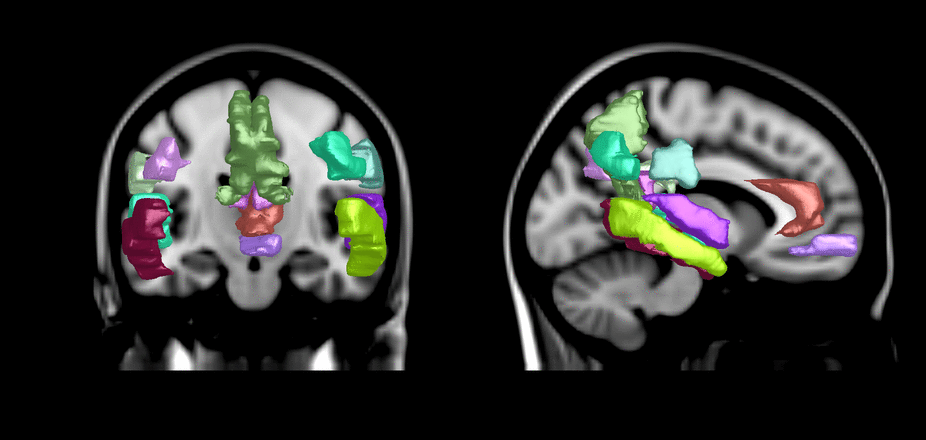
\includegraphics[width=0.8\textwidth]{3_covtraj/figs/PiBROIsMontage.png}
  \caption{\label{fig:pibrois}16 Positron Emission Tomography (PET) regions.}
\end{figure*}

\newpage

\subsubsection*{DTI Imaging}
Diffusion tensor imaging is used to measure the restricted diffusion of water through and about regions of the brain. The 48 regions here are the aggregated measurements of total rates of diffusion for each voxel in that region. The two measurements, Fractional Anisotropy (FA) and Mean Diffusivity (MD) collectively well describe the diffusion in a specific region. The following is the full list of regions used in our analysis. Regions that spanned across both the left and right sides of the brain are indicated as such, and were treated as separate and independent in our analyses. 
{\small
\begin{multicols}{2}
\begin{enumerate}
\item Middle cerebellar peduncle
\item Pontine crossing tract (a part of MCP)
\item Genu of corpus callosum
\item Body of corpus callosum
\item Splenium of corpus callosum
\item Fornix (column and body of fornix)
\item Corticospinal tract R/L
\item Medial lemniscus R/L
\item Inferior cerebellar peduncle R/L
\item Superior cerebellar peduncle R/L
\item Cerebral peduncle R/L
\item Anterior limb of internal capsule R/L
\item Posterior limb of internal capsule R/L
\item Retrolenticular part of internal capsule R/L
\item Anterior corona radiata R/L
\item Superior corona radiata R/L
\item Posterior corona radiata R/L
\item Posterior thalamic radiation (include optic radiation) R/L
\item Sagittal stratum (include inferior longitidinal fasciculus and inferior fronto-occipital fasciculus) R/L
\item External capsule R/L
\item Cingulum (cingulate gyrus) R/L
\item Cingulum (hippocampus) R/L
\item Fornix (cres) / Stria terminalis (can not be resolved with current resolution) R/L
\item Superior longitudinal fasciculus R/L
\item Superior fronto-occipital fasciculus (could be a part of anterior internal capsule) R/L
\item Uncinate fasciculus R/L
\item Tapetum R/L
\end{enumerate}
\end{multicols}
}
\begin{figure*}
\centering
  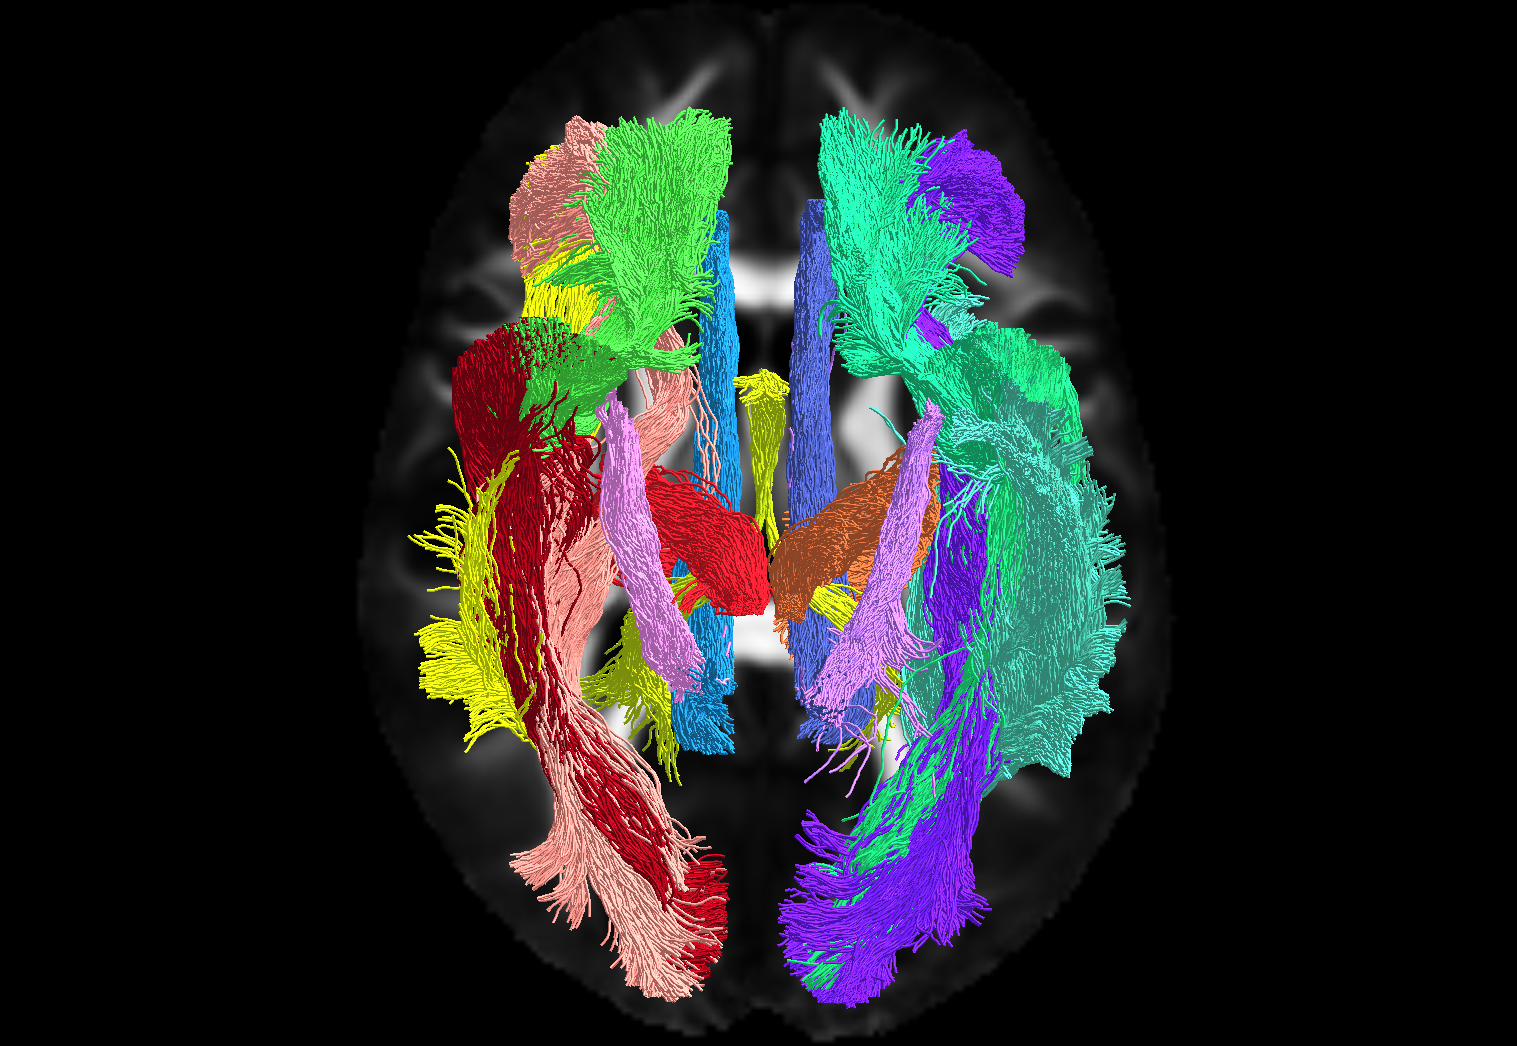
\includegraphics[width=0.32\textwidth]{3_covtraj/figs/majorDTI_FA/screenshot0001.png}
  %
  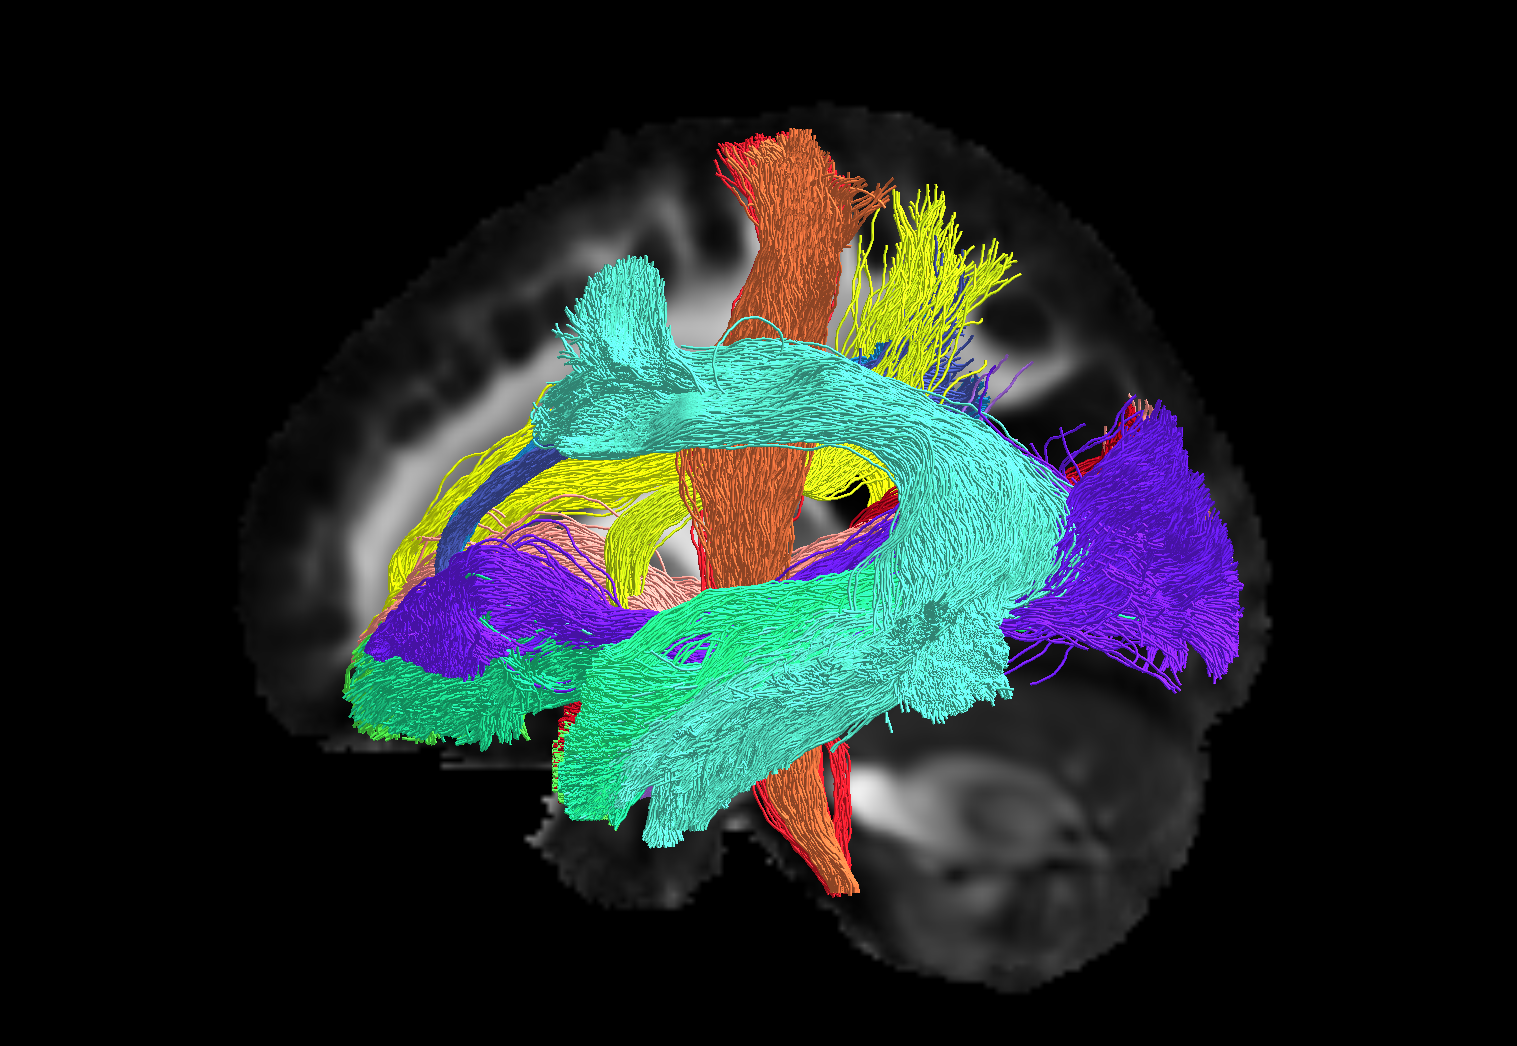
\includegraphics[width=0.32\textwidth]{3_covtraj/figs/majorDTI_FA/screenshot0002.png}
  %
  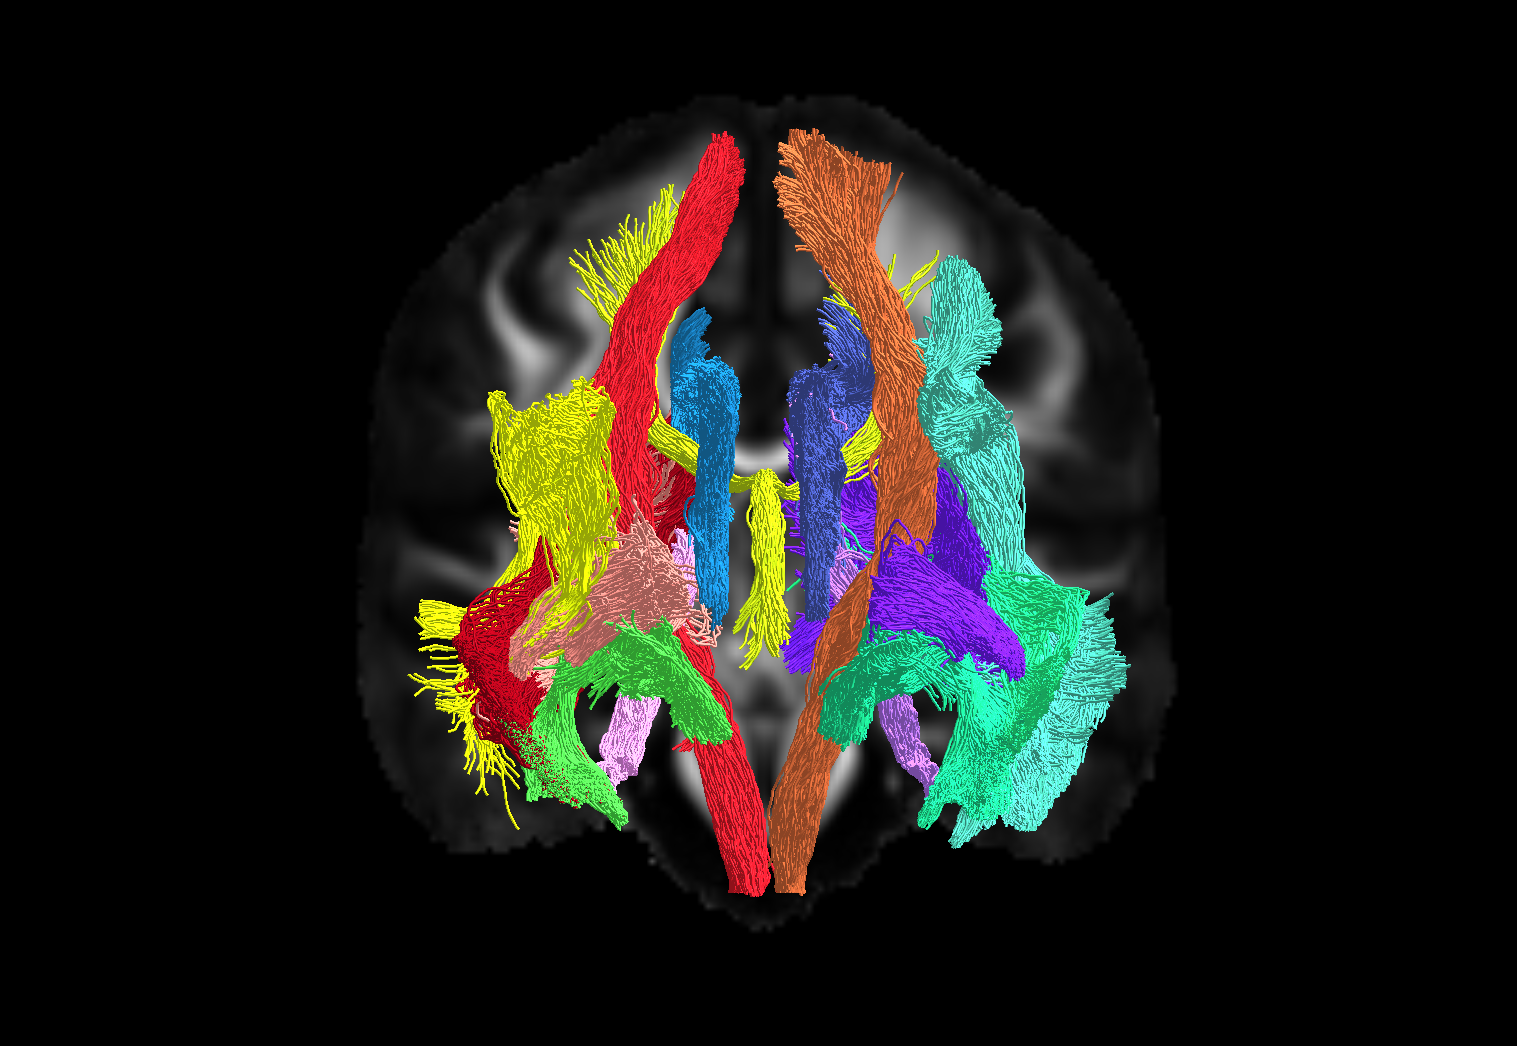
\includegraphics[width=0.32\textwidth]{3_covtraj/figs/majorDTI_FA/screenshot0003.png}
  \caption{\label{fig:majorDTI}17 major DTI fiber bundles measured using Fractional Anisotropy (FA). The 48 selected for our analysis include a subset of these, which have been identified as critical regions that signal the beginnings of cognitive impairment.}
\end{figure*}

\newpage

\subsubsection*{Cognitive Evaluations}
The battery of cognitive test scores in our analysis included a breadth of evaluations chosen specifically for their coverage of various measures of cognition. Among all tests given to the cohort, the following 17 were selected by expert clinicians and researchers in the field for their coverage and their potential value in understanding trends across groups.
{\small
\begin{multicols}{2}
\begin{enumerate}
\item WAIS-III Digit Span Forward Raw Score
\item WAIS-III Digit Span Backward Raw Score
\item WAIS-III Letter-Number Sequencing Raw Score
\item COWAT CFL Score
\item Boston Naming Test Total Score
\item RAVLT Learning Trial A1 Raw Score
\item RAVLT Learning Trial A2 Raw Score
\item RAVLT Learning Trial A3 Raw Score
\item RAVLT Learning Trial A4 Raw Score
\item RAVLT Learning Trial A5 Raw Score
\item RAVLT Learning Trial A6 Raw Score
\item RAVLT Delayed Recall Raw Score
\item Stroop Word/Color-Word Scaled Score
\item Trail-Making Test Part A
\item Trail-Making Test Part B
\item Clock Drawing Test Score
\item Center for Epidemiologic Studies Depression Scale Score
\end{enumerate} 
\end{multicols}
}

{\bf WAIS-III.} This is the most widely used IQ test. The Digit Span examination is specifically meant to evaluate the working memory of an individual. Participants are required to attempt to recall a series of numbers in order, both forwards and backwards. Letter-Number sequencing reflects a similar idea, but with a mix of both numbers and letters in increasing and alphabetical order, and is meant to be an indicator of more complex mental control \cite{wechsler2014wechsler}.

{\bf Rey Auditory Visual Learning Test.} This test is specifically meant to evaluate all aspects of memory. Each trial evaluates a different type of memory, ranging from short-term and working memory to procedural and episodic memory. \cite{schmidt1996rey}.

{\bf Trail-Making Test.} This is a very popular test in providing information about executive function in the brain. The test consists of drawing lines among a randomly generated set of points in a square, where each point is labeled with a number. In Part A, participants must `connect the dots' in increasing numerical order, and in Part B in increasing numerical and alphabetical order. The score on the test is primarily dictated by the time in seconds it takes to complete the task for 25 of these `dots.' More background information and normative analyses can be found in \cite{tombaugh2004trail}.

Other tests similarly measure various cognitive function. While the Depression Scale Score did not crop up in any of our analyses here, it has been shown that depression is strongly associated with AD-related decline \cite{wragg1989overview}.